\documentclass[fontset=ubuntu]{ctexart}


% ------- 导入包 ------- %
\usepackage{hyperref}
\usepackage{fancyhdr}
\usepackage{tabularx}
\usepackage{graphicx}
\usepackage{amsmath}

% ------- 页眉页脚设置 ------- %
\pagestyle{fancy}
\fancyhf{}
\fancyfoot[C]{\thepage}
\renewcommand{\headrulewidth}{0pt}
\renewcommand{\footrulewidth}{0pt}


% ------- 图片编号 ------- %

% ------- 标题页 ------- % 
\title{红酒质量分析报告}
\author{回归分析小组}
\date{\today}


% ------- 主文档 ------- %
\begin{document}

    % ------- 标题页 ------- %
    \maketitle
    \thispagestyle{empty}
    \newpage

    % ------- 目录页 ------- %
    \tableofcontents
    \thispagestyle{empty}
    \newpage
    \setcounter{page}{1} % 重置页码

    % ------- 正文 ------- %
    \section{问题背景}
        随着酒类产品在市场上的广泛受欢迎,对于酒的质量和特征的深入了解变得至关重要。为了更好地了解酒的品质,我们进行了一项回归分析,重点关注了酒的酸度,二氧化硫($SO_2$)含量等特征。这些特征在很大程度上影响了酒的口感、风味和保存能力。 

    \section{数据说明}
        我们通过 \href{https://archive.ics.uci.edu/dataset/186/wine+quality}{UC Irvine}仓库下载了红酒数据,数据集中的特征包含酒的各类化学成分指标以及酒的品质评价。其中,成分指标,如$pH$值、$SO_2$含量、残糖量等通过物理化学检测得出;酒的品质由专业品酒师做出评价。(每个样本由三个品酒师做出评价,每个人的评分为$0$(差)到$10$(好)的一个整数,最终评价取三人的中位数)。红酒共$1599$条数据,其中不含缺失值,共记录了$12$个特征,特征说明如 \ref{tab:features} 所示。

        \begin{table}[htbp]
            \centering
            \caption{酒的特征说明}
            \vspace{5pt}
            \begin{tabular}{cccc}
                \hline
                变量名 & 中文含义 & 变量类型 & 单位 \\
                \hline
                fixed acidity & 固定酸度 & 连续型变量 & g/L \\
                Volatile Acidity & 挥发性酸度 & 连续型变量 & g/L \\
                Citric Acid & 柠檬酸 & 连续型变量 & g/L\\
                Residual Sugar & 残糖 & 连续型变量 & g/L \\
                Chlorides & 氯化物 & 连续型变量 & g/L\\
                Free Sulfur Dioxide & 游离二氧化硫 & 连续型变量 & g/L \\
                Total Sulfur Dioxide & 总二氧化硫 & 连续型变量 & g/L \\
                Density & 密度 & 连续型变量 & g/mL \\
                pH &  葡萄酒的pH值 & 连续型变量 & \\
                Sulphates & 硫酸盐 & 连续型变量 & g/L \\
                Alcohol & 醇度 & 连续型变量 & \% \\
                Quality & 酒品 & 离散型变量 & \\ 
                \hline
            \end{tabular}
            \label{tab:features}
        \end{table}

    \section{描述性统计}
        \subsection{数值特征}
        对数据的初步描述如表 \ref{tab:description1-4},表\ref{tab:description5-8}和表\ref{tab:description9-12} 所示,包含平均值、最小值、最大值、中位数。
        \begin{table}[ht]
            \centering
            \caption{数据描述1-4}
            \vspace{5pt}
            \begin{tabular}{lllll}
                \hline
                fixed.acidity & volatile.acidity &  citric.acid & residual.sugar \\ 
                \hline
                Min.   : 4.60   & Min.   :0.1200   & Min.   :0.000   & Min.   : 0.900   \\ 
                1st Qu.: 7.10   & 1st Qu.:0.3900   & 1st Qu.:0.090   & 1st Qu.: 1.900   \\ 
                Median : 7.90   & Median :0.5200   & Median :0.260   & Median : 2.200   \\ 
                Mean   : 8.32   & Mean   :0.5278   & Mean   :0.271   & Mean   : 2.539   \\ 
                3rd Qu.: 9.20   & 3rd Qu.:0.6400   & 3rd Qu.:0.420   & 3rd Qu.: 2.600   \\ 
                Max.   :15.90   & Max.   :1.5800   & Max.   :1.000   & Max.   :15.500   \\ 
               \hline
            \end{tabular}
            \label{tab:description1-4}
        \end{table}

        \begin{table}[ht]
            \centering
            \caption{数据描述5-8}
            \vspace{5pt}
            \begin{tabular}{lllll}
                \hline
                chlorides & free.sulfur.dioxide & total.sulfur.dioxide &    density \\ 
                \hline
                Min.   :0.01200   & Min.   : 1.00   & Min.   :  6.00   & Min.   :0.9901   \\ 
                1st Qu.:0.07000   & 1st Qu.: 7.00   & 1st Qu.: 22.00   & 1st Qu.:0.9956   \\ 
                Median :0.07900   & Median :14.00   & Median : 38.00   & Median :0.9968   \\ 
                Mean   :0.08747   & Mean   :15.87   & Mean   : 46.47   & Mean   :0.9967   \\ 
                3rd Qu.:0.09000   & 3rd Qu.:21.00   & 3rd Qu.: 62.00   & 3rd Qu.:0.9978   \\ 
                Max.   :0.61100   & Max.   :72.00   & Max.   :289.00   & Max.   :1.0037   \\ 
                \hline
            \end{tabular}
            \label{tab:description5-8}
        \end{table}

        \begin{table}[ht]
            \centering
            \caption{数据描述9-12}
            \vspace{5pt}
            \begin{tabular}{lllll}
                \hline
                pH &   sulphates &    alcohol &    quality \\ 
                \hline
                Min.   :2.740   & Min.   :0.3300   & Min.   : 8.40   & Min.   :3.000   \\ 
                1st Qu.:3.210   & 1st Qu.:0.5500   & 1st Qu.: 9.50   & 1st Qu.:5.000   \\ 
                Median :3.310   & Median :0.6200   & Median :10.20   & Median :6.000   \\ 
                Mean   :3.311   & Mean   :0.6581   & Mean   :10.42   & Mean   :5.636   \\ 
                3rd Qu.:3.400   & 3rd Qu.:0.7300   & 3rd Qu.:11.10   & 3rd Qu.:6.000   \\ 
                Max.   :4.010   & Max.   :2.0000   & Max.   :14.90   & Max.   :8.000   \\ 
                \hline
            \end{tabular}
            \label{tab:description9-12}
            \end{table}
        
        \clearpage
        \subsection{因变量描述}
            首先通过直方图观察酒品分布情况,可以发现,数据主要集中在$5, 6$。 
            \begin{figure}[htbp]
                \centering
                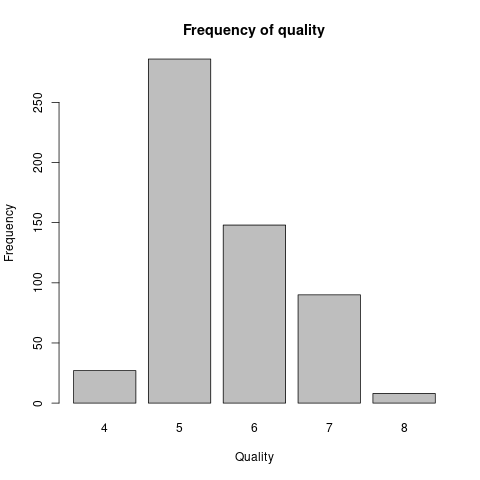
\includegraphics[width=0.8\textwidth]{../figures/quality-frequency.png}
                \label{fig:quality}
                \caption{酒品数据分布}
            \end{figure}

        \subsection{自变量描述}
            我们通过自变量的分布图和自变量与酒品的箱线图对其进行描述。下面展示部分具有代表性的数据。
            \clearpage
            \subsubsection{硫酸盐(Sulphates)}
                硫酸盐的分布图和关于酒品的箱线图如图所示。
                \begin{figure}[htbp]
                    \centering
                    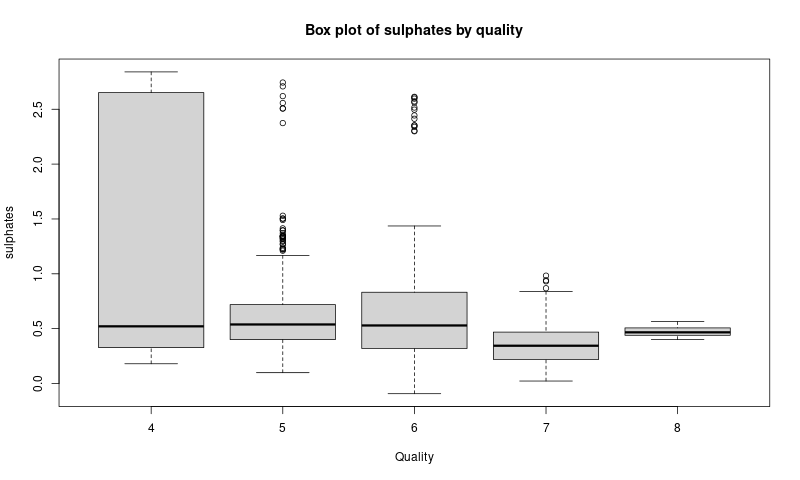
\includegraphics[width=0.8\textwidth]{../figures/sulphates-plot.png}
                    \label{fig:sulphates}
                    \caption{硫酸盐分布及箱线图}
                \end{figure}

            \subsubsection{酒精(Alcohol)}
                酒精含量的分布图和关于酒品的箱线图如图所示。
                \begin{figure}[htbp]
                    \centering
                    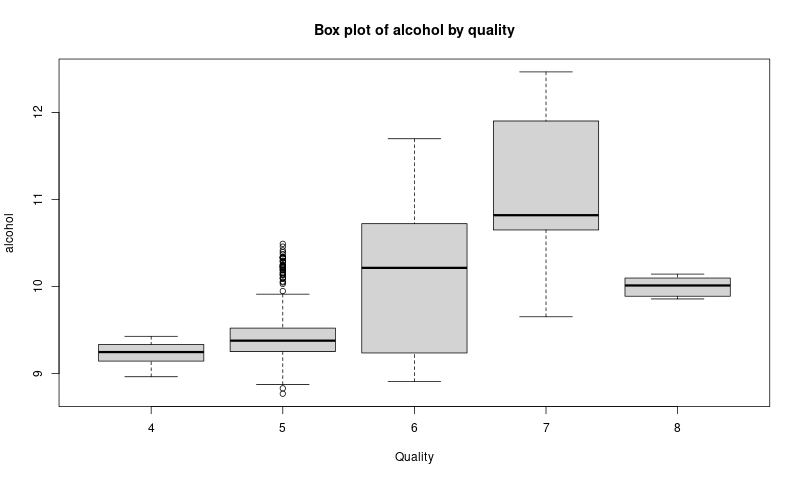
\includegraphics[width=0.8\textwidth]{../figures/alcohol-plot.png}
                    \label{fig:alcohol}
                    \caption{酒精分布及箱线图}
                \end{figure}
            
            \subsubsection{总二氧化硫(Total Sulfur Dioxide )}
                总二氧化硫含量的分布图和关于酒品的箱线图如图所示。
                \begin{figure}[htbp]
                    \centering
                    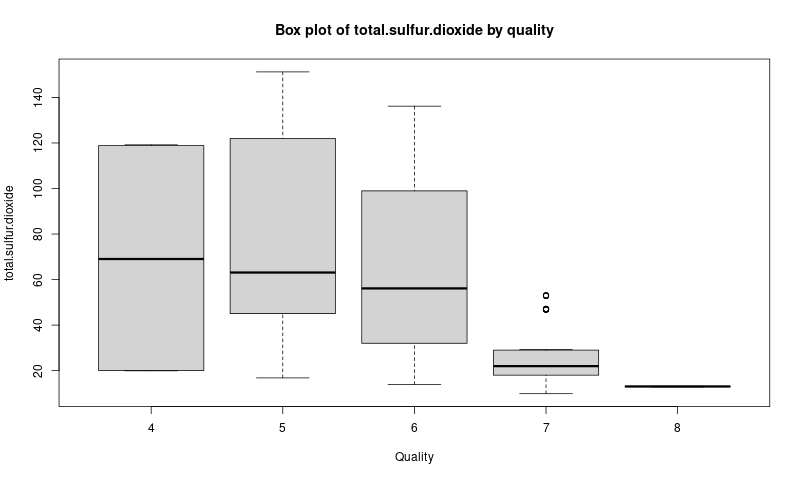
\includegraphics[width=0.8\textwidth]{../figures/total.sulfur.dioxide-plot.png}
                    \label{fig:total.sulfur.dioxide}
                    \caption{总二氧化硫分布及箱线图}
                \end{figure}   

            \subsubsection{氯化物(Chlorides)}
            氯化物含量的分布图和关于酒品的箱线图如图所示。
            \begin{figure}[htbp]
                \centering
                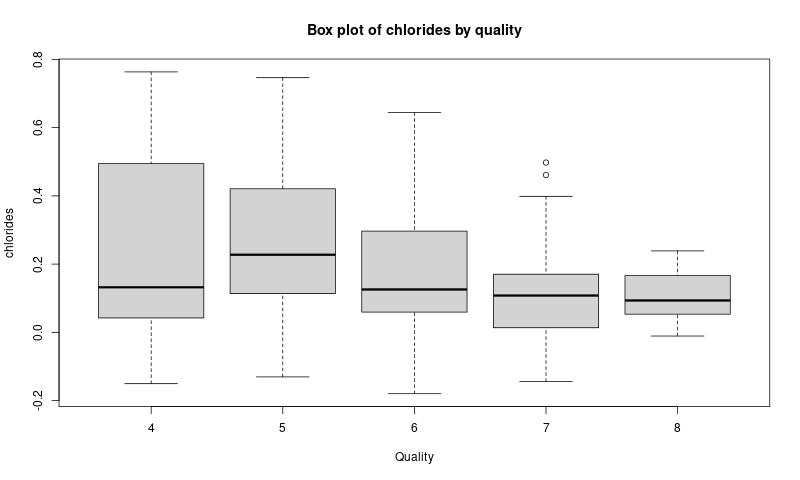
\includegraphics[width=0.8\textwidth]{../figures/chlorides-plot.png}
                \label{fig:chlorides}
                \caption{氯化物分布及箱线图}
            \end{figure} 
            
    \section{数据建模}
        我们首先使用线性模型全模型,通过红酒的化学成分特征,对酒品进行回归分析。

        \subsection{全模型}

    \section{结论及建议}

    \newpage
    %\bibliographystyle{plain}
    %\bibliography{ref} 

\end{document}